
\documentclass[../main.tex]{subfiles}

\begin{document}

\subsection*{Leaf Logical Forms corpus}

We developed annotation guidelines for the LLF corpus using a simplification of entities and relations from the preceding LCT corpus\cite{dobbins2022leaf}. Generally speaking, LCT \textit{entities} correspond to logical form \textit{functions}, while LCT \textit{relations} correspond to logical form \textit{predicates}. For example, the LCT \textit{Condition} entity has a corresponding \textit{cond()} function, while the \textit{Num-Filter} relation has a corresponding \textit{.num\_filter()} predicate. The LLF annotation guidelines can be found at \url{https://github.com/ndobb/clinical-trials-seq2seq-annotation/wiki}.

We also hypothesized that the performance of predicting logical forms could likely be improved by replacing "raw" tokens in each eligibility criteria with corresponding logical form names derived from named entities from the LCT corpus. For example, given the eligibility criterion: \\

"\textit{Diabetics who smoke}", \\

\noindent we would replace the named entities for "Diabetics" and "smoke": \\ 

\textit{cond("Diabetics") who obs("smoke")} \\

\noindent using \textit{Condition} and \textit{Observation} annotations in the LCT corpus. We call this substituted text an "augmented" eligibility criteria. The augmented criteria syntax reshapes named entities to more closely resemble expected logical form syntax and allows us to leverage the LCT corpus for logical form transformation.

Creation and annotation of the LLF corpus proceeded in the following steps:

\begin{enumerate}
    \item We randomly chose 2,000 lines of eligibility criteria from the LCT corpus, limited to only criteria which included at least one named entity and which were not annotated as hypothetical criteria.
    \item  Each annotation file consists of the text "EXC" if exclusion or "INC" if inclusion (line 1), an original "raw" eligibility criteria (line 3), an augmented eligibility criteria (line 5), and an (initially blank) expected logical form equivalent to annotate (line 7). An example annotation is shown in Figure \ref{fig_annotation_example}.
    \item 3 informatics graduate students met weekly for 2 months to review annotations. Annotators were initially trained on 20 triple-annotated training annotations. 
    \item After training, each annotator was assigned a batch of 100 sentences (one per file) and tasked with writing a logical form version of each.
    \item After each batch was completed, we executed a quality control script to parse each logical form annotation to ensure consistency. Any syntax errors were reported to and corrected by the annotators.
    \item Annotators received additional batches of files to annotate until all 2,000 single-annotated annotations had been completed.
\end{enumerate}

\begin{figure}[h!]
  \centering
  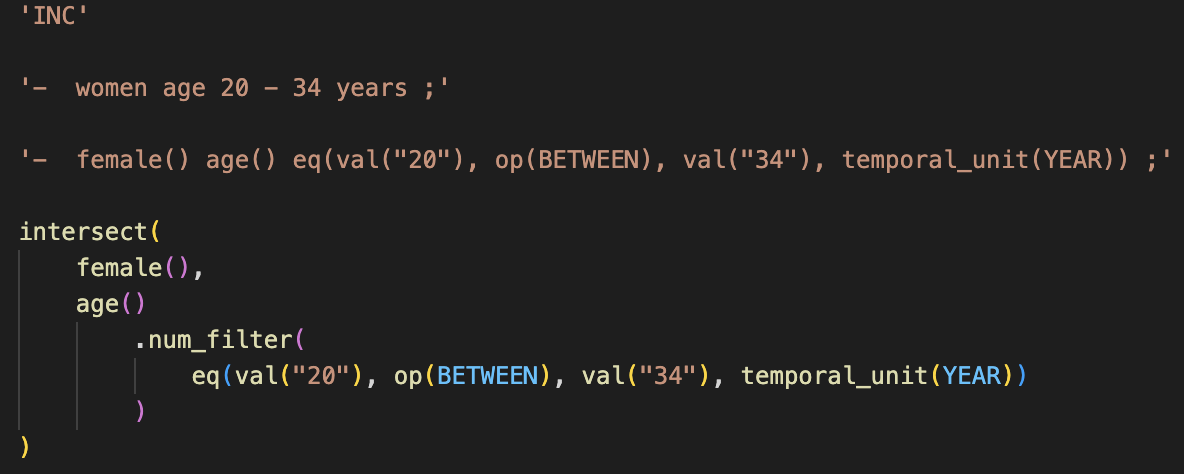
\includegraphics[scale=0.7]{figures/leafai_appdx_annotation_example.png}  
  \caption{A example LLF corpus annotation. The annotation file is saved in JavaScript (.js) format, which enables syntax highlighting and validation to assist annotators. Whether a given criterion was an inclusion or exclusion criteria is indicated at the top, followed by the original raw text, then augmented text. The final annotated logical forms are shown last.}
\label{fig_annotation_example}
\end{figure}

After annotations were completed, we experimented with predicting logical forms by fine-tuning T5 \cite{raffel2020exploring} Seq2Seq models. The T5 architecture and pre-trained models are widely used for and achieve at or near state-of-the-art for many machine translation and semantic parsing tasks. 

Following earlier work on task-oriented dialog semantic parsing structures in the domain of digital assistants, we also experimented using various alternative input-output syntax styles from our original logical forms:

\begin{enumerate}
    \item \textbf{Shift-Reduce}. Einolghozatic \textit{et al} \cite{einolghozati2019improving} used square brackets instead of parentheses and blank spaces instead of commas. We followed Rongali \textit{et al's} suggestion to add a trailing repeat of function names to improve performance.
    \item \textbf{Pointer}. Rongali \textit{et al} found that replacing input tokens with "$@ptr_{index}$", where \textit{index} corresponds to a token's sequential position in the input text improved performance in their semantic parsing task. We modified this approach by omitting the characters "ptr" and using the sequential position of the quoted span as our index rather than individual token positions.
\end{enumerate}

We used a randomly sorted 70/20/10 train/test/validation split of the LFF corpus to fine-tune the pretrained T5$_{base}$ model using combinations of these syntax styles. We call our gold standard annotated logical form syntax "Standard" style. Example inputs, outputs, and training results are shown in Table \ref{tbl_llf_corpus}. 

\begin{table}[h!]
    \footnotesize
    \centering
    \def\arraystretch{1.4}
\definecolor{gray}{RGB}{230,230,230}
\begin{tabular}{m{2.5cm} l l l l}
    \toprule
    \textbf{Syntax Style} & \textbf{Example Input} & \textbf{Example Logical Form} & \textbf{BLEU} & \textbf{ROUGE-L} \\
    \midrule
    \arrayrulecolor{gray}
    Raw-text→ Standard       
       & Diabetics who smoke                     
       & $\makecell[cl]{intersect(\\\mathrm{\ \ \ }cond("Diabetics"), \\\mathrm{\ \ \ }obs("smoke")\\)}$
       & 78.7
       & 79.1 \\
    \midrule
    Standard  
       & cond("Diabetics") who obs("smoke")           
       & $\makecell[cl]{intersect(\\\mathrm{\ \ \ }cond("Diabetics"), \\\mathrm{\ \ \ }obs("smoke")\\)}$
       & \textbf{93.5}
       & \textbf{92.3} \\
    \midrule
    Standard+ Pointer
       & cond(@1) who obs(@2)                          
       & $\makecell[cl]{intersect(\\\mathrm{\ \ \ }cond(@1), \\\mathrm{\ \ \ }obs(@2)\\)}$
       & 93.3
       & 91.2 \\
    \midrule
    Shift-Reduce              
       & [cond "Diabetics" cond] who [obs "smoke" obs] 
       & $\makecell[cl]{[intersect\\\mathrm{\ \ \ }[cond\mathrm{\ }"Diabetics"\mathrm{\ }cond]\\\mathrm{\ \ \ }[obs\mathrm{\ }"smoke"\mathrm{\ }obs]\\ intersect]}$
       & 89.8
       & 91.7 \\
    \midrule
    Shift-Reduce+ Pointer     
       & [cond @1 cond] who [obs @2 obs]               
       & $\makecell[cl]{[intersect\\\mathrm{\ \ \ }[cond\mathrm{\ }@1\mathrm{\ }cond]\\\mathrm{\ \ \ }[obs\mathrm{\ }@2\mathrm{\ }obs]\\ intersect]}$
       & 89.4
       & 90.4 \\
    \bottomrule       
\end{tabular}
    \caption{Example inputs and logical form syntax styles with fine-tuning performance results using the T5$_{base}$ model.}
    \label{tbl_llf_corpus}
\end{table} 

We found that our Standard logical forms achieved the highest performance using both BLEU \cite{lin2004rouge} and ROUGE-L \cite{ callison2006re} scores, two commonly used metrics in measuring Seq2Seq performance. Replacing raw tokens with function names corresponding to named entities also significantly improved performance (+14.7\%, comparing raw text to Standard input styles), demonstrating that leveraging the LCT corpus to generate augmented text achieved relatively high performance (> 93\% BLEU score) for this task. As it was the highest-performing syntax style and also the most straightforward to parse, we chose to use the Standard logical form style as our IR for LeafAI.

\end{document}